\def\layersep{2.5cm}

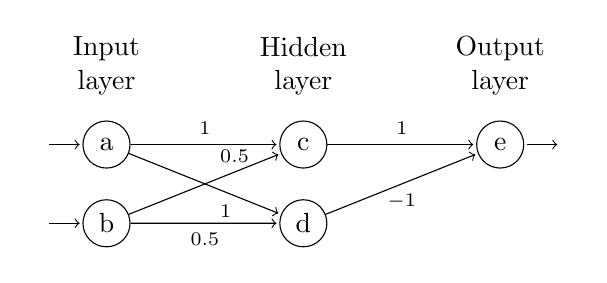
\begin{tikzpicture}[shorten >=1pt,->,draw=black, node distance=\layersep,
	every edge/.append style={nodes={font=\scriptsize}}]
    \tikzstyle{every pin edge}=[<-,shorten <=1pt]
    \tikzstyle{neuron}=[circle,draw=black,minimum size=17pt,inner sep=0pt]
    \tikzstyle{input neuron}=[neuron];
    \tikzstyle{output neuron}=[neuron];
    \tikzstyle{hidden neuron}=[neuron];
    \tikzstyle{annot} = [text width=4em, text centered]

    % Draw the input layer nodes
    %\foreach \name / \y in {1,...,2}
    % This is the same as writing \foreach \name / \y in {1/1,2/2,3/3,4/4}
        \node[input neuron, pin=left:] (I-1) at (0,-1) {a};
        \node[input neuron, pin=left:] (I-2) at (0,-2) {b};

    % Draw the hidden layer nodes
    %\foreach \name / \y in {1,...,2}
        \node[hidden neuron] (H-1) at (\layersep,-1 cm) {c};
        \node[hidden neuron] (H-2) at (\layersep,-2 cm) {d};

    % Draw the output layer node
    \path[yshift=0.5cm]
    		node[output neuron,pin={[pin edge={->}]right:}, right of=H-1] (O) {e};

    % Connect every node in the input layer with every node in the
    % hidden layer.    
    \path (I-1) edge node[above]{$1$} (H-1);
    \path (I-1) edge node[above=10pt,right=2pt]{$0.5$} (H-2);
    \path (I-2) edge node[below=10pt,right=2pt]{$1$} (H-1);
    \path (I-2) edge node[below]{$0.5$} (H-2);

    % Connect every node in the hidden layer with the output layer
    \path (H-1) edge node[above]{$1$} (O);
    \path (H-2) edge node[below]{$-1$} (O);

    % Annotate the layers
    \node[annot,above of=H-1, node distance=1cm] (hl) {Hidden layer};
    \node[annot,left of=hl] {Input layer};
    \node[annot,right of=hl] {Output layer};
\end{tikzpicture}